\documentclass[11pt]{article}
% NSF PAPPG Ch. 2 §B.2: font ≥11pt, margins ≥1in, ≤6 lines/inch.
% No hyperlinks in Project Description body (Research.gov constraint).

\usepackage{amsmath}
\usepackage{bm}
\usepackage{color}
\usepackage{hyperref}
\usepackage{graphicx}
\usepackage{wrapfig}
\usepackage{subcaption}
\usepackage{vmargin}
\usepackage{mathrsfs}
\usepackage{float}
\usepackage{tabularx}
\usepackage{booktabs} 
\usepackage{longtable}
\usepackage{ltablex}
\usepackage[svgnames]{xcolor}
\usepackage[most]{tcolorbox}
\usepackage{enumitem}
\usepackage{titlesec}
\usepackage{caption}
\usepackage{colortbl}
\usepackage[numbers,square,sort&compress]{natbib}

% ── Colors ───────────────────────────────────────────────────────────────────
\definecolor{mycmykcolor}{cmyk}{0.45,0.30,0.20,0}
\definecolor{secondary}{cmyk}{0,0,0,0.20}

% ── Section formatting ────────────────────────────────────────────────────────
\titleformat{\section}[runin]{\normalfont\bfseries}{\thesection}{1em}{}[:]
\titlespacing*{\section}{0pt}{\baselineskip}{1ex}
\titleformat{\subsection}[runin]{\normalfont\bfseries}{\thesubsection}{1em}{}[:]
\titlespacing*{\subsection}{0pt}{\baselineskip}{1ex}

% ── Page layout ───────────────────────────────────────────────────────────────
\bibliographystyle{unsrtnat}
\hypersetup{hidelinks,colorlinks=false,urlcolor=black}
\hypersetup{draft}
\setpapersize{USletter}
\setmarginsrb{1in}{1in}{1in}{1in}{0pt}{0mm}{0pt}{0mm}
\pretolerance=5000
\tolerance=9000
\graphicspath{{images/}}

\newcommand{\placeholder}[1]{\textcolor{red}{[\textbf{PLACEHOLDER:} #1]}}
\newcommand{\pseudodot}{{\lower 2.4pt\hbox{$\cdot$}}}

\begin{document}
% \pagestyle{empty} % turn back on for nsf
\setlength{\baselineskip}{12.6pt}
\setlength{\normalbaselineskip}{12.6pt}

% ============================================================
%  PROJECT GOALS BOX
% ============================================================

\begin{tcolorbox}[colback=mycmykcolor, colframe=black, boxrule=1pt, coltext=black]
\textbf{Project goals:}
Small, repeatedly-flooded municipalities with pre-code building stock have no
engineering tool to evaluate whether community-scale drainage investment or distributed
building hardening better reduces flood damage.
Here, we propose a closed-loop cyber-physical system (CPS) organized around the following four coupled layers:
the \textbf{physical layer} (pre-code load-bearing masonry and timber structures,
absent from existing fragility frameworks);
the \textbf{sensing layer} (USGS stream gauges and NOAA precipitation for operational
use, with ICEYE commercial Synthetic Aperture Radar (SAR) providing building-level inundation duration and depth for one-time model calibration, and open Sentinel-1 SAR providing broader flood-extent context);
the \textbf{cyber layer} (a Bayesian framework fusing a GIS-parameterizable hydrological
mass balance model with community-elicited priors on inundation duration and depth); and
the \textbf{decision layer} (a co-developed three-mode interface supporting retrofit
planning, pre-storm resource staging, and post-event model updating).
\textbf{RQ1} (Napolitano, Wauthier, and Busse) asks whether this CPS provides
decision-adequate probabilistic flood damage assessments for small municipalities
with pre-code building stock, enabling evaluation of building-specific hardening
and community-scale drainage investments without resource-intensive simulation,
and pre-storm resource staging from forecast precipitation inputs.
\textbf{RQ2} (Napolitano with input from all PIs) asks under what conditions locally held
community knowledge, entered as Bayesian calibration priors, improves damage
assessments relative to a GIS-only baseline, and where it functions as a substitute
versus complement to geospatial data.
The defining intellectual contribution is treating community knowledge as a structural
calibration input whose epistemic contribution is directly measurable against a
geospatial data baseline.
\end{tcolorbox}
\vspace{-0.5cm}

\begin{wrapfigure}{r}{0.45\textwidth}

\includegraphics[width=0.45\textwidth]{images/img.jpg}
\captionsetup{justification=centering,singlelinecheck=false,font=small}
\caption{Four-layer CPS architecture. The operational sensing layer uses free
USGS and NOAA data; ICEYE commercial SAR provides building-level ground truth
for one-time model calibration only, with open Sentinel-1 SAR providing
broader flood-extent context.}
\label{fig:cps_arch}
\end{wrapfigure}
\normalsize

% ============================================================
%  STATUS QUO
% ============================================================

\section{Status quo}
Small, aging communities at the confluence of riverine flood hazard and pre-code
building stock face a resilience challenge that no existing engineering framework
is designed to address.
Across the northeastern United States and Appalachian corridor, thousands of towns
share this profile: riverine flood exposure with multi-day inundation durations,
dense historic cores of load-bearing masonry and timber construction built before
modern building codes, and institutional capacity below the threshold required for
hydrodynamic simulation \cite{placeholder_nfip}.
FEMA's National Flood Insurance Program enrolls over 22,000 communities nationwide;
the subset in this region with significant pre-1940 building stock, no sustained
in-house hydraulic modeling capacity, and a history of repeated riverine flooding
numbers in the thousands \cite{placeholder_acs}.
For these communities, every flood event surfaces the same unresolved question:
where do limited retrofit dollars belong?

That question involves two distinct decisions that existing frameworks cannot place
on the same probabilistic basis.
The first is the building-scale question: which structures sustain damage severe enough
to justify investment in flood barriers, foundation waterproofing, or structural
hardening?
The second is the community-scale question: would a drainage investment, such as a
retention basin, channel improvement, or permeable infrastructure upgrade, reduce
building damage enough across the community to justify its cost over distributed
individual retrofits?
Answering the second question requires connecting upstream drainage decisions to
downstream building damage probabilities through a physical model of the relevant
building stock. No such model exists for small communities with pre-code building
stock, and no existing framework allows these two decisions to be compared on a comparable probabilistic basis.

Existing flood damage assessment tools were designed for the resources and building
stocks of larger municipalities.
Hydrodynamic simulation pipelines such as HEC-RAS and LISFLOOD-FP require calibrated
hydraulic models, high spatial resolution topographic data, and sustained technical capacity
that small towns cannot maintain. % becca add refs
Damage functions in HAZUS and FEMA P-58 are built around post-1945 construction
archetypes; pre-code load-bearing masonry and timber structures, the dominant building
type in repeatedly-flooded historic downtowns, are absent from existing fragility
frameworks. % becca add refs
The most authoritative federal guidance on infrastructure functional recovery, NIST
SP~1310 \cite{davis2024nist}, explicitly acknowledges that its framework is too
complex for smaller agencies with limited resources and funding, and calls for
simplifications that can be implemented at the capacity levels of smaller
organizations \cite[Sec.~6.1.3]{davis2024nist}.
Emergency managers, historic preservation officials, and building owners in these
communities have no engineering tool that translates a flood event into building-specific
guidance on where limited retrofit dollars belong.

\begin{wrapfigure}{r}{0.45\textwidth}
\vspace{-0.4cm}

\includegraphics[width=0.45\textwidth]{images/img.jpg}
\captionsetup{justification=centering,singlelinecheck=false,font=small}
\vspace{-0.9cm}
\caption{\placeholder{Pre-code load-bearing masonry buildings in Montpelier.}}
\label{fig:precode}
\vspace{-0.3cm}
\end{wrapfigure}

These buildings degrade under extended inundation through duration-governed mechanisms
including mortar softening, masonry unit saturation, and rising damp-driven cohesion
loss that current assessment tools neither observe nor model.
Existing community flood resilience frameworks are predominantly top-down in design,
built around standardized data collection and technical modeling pipelines that
resource-constrained localities cannot sustain.
Community-generated data and locally held knowledge offer an underutilized pathway
to resilience assessment in these settings; no existing framework provides a
mechanism for communities to contribute that knowledge to engineering-grade
probabilistic assessments.

\vspace{-10pt}
\subsection{Research questions and intellectual merit}

\begin{itemize}[leftmargin=1.5em,itemsep=0pt]
\item \textbf{RQ1 (Napolitano, Wauthier, and Busse):} Can a CPS coupling a
GIS-parameterizable mass balance model with community knowledge provide
decision-adequate building-level flood damage assessments for small municipalities
with pre-code building stock, supporting both retrofit allocation and pre-storm
resource staging without hydraulic simulation?
\item \textbf{RQ2 (Napolitano with input from all PIs):} Under what conditions does locally
held community knowledge, entered as Bayesian calibration priors, improve flood
damage assessment accuracy and calibration relative to a GIS-only baseline, and
where does it function as a substitute versus complement to geospatial data?
\end{itemize}

These questions together span three scientific contributions.
First, this research establishes whether a GIS-parameterizable mass balance model,
fused with community knowledge in a Bayesian framework, can provide decision-adequate
building-level flood damage assessment for retrofit allocation without hydrodynamic
simulation; it advances a generalizable CPS architecture principle by demonstrating
that free, nationally available geospatial data fused with community knowledge is
sufficient for the specific investment decisions small municipalities face, including
pre-storm decisions made before water rises.
Second, existing fragility frameworks take depth as the governing input and are
structurally incompatible with a CPS cyber layer that produces duration estimates;
this research produces the first empirically derived, duration-dependent fragility
surfaces for pre-code load-bearing masonry archetypes, calibrated on 271 buildings
from the 2023 Montpelier flood and validated on the held-out 2024 event.
Third, it characterizes the conditions under which locally held community knowledge,
entered as Bayesian priors, improves model accuracy and calibration relative to a
GIS-only baseline, and what the pattern of improvement reveals about where community
knowledge and geospatial data are substitutes versus complements in CPS calibration.

\begingroup
\footnotesize
\begin{tabularx}{\textwidth}{|X|X|X|X|}
\caption{Summary of research gaps, objectives, approaches, and outcomes%
         \label{tab:research_summary}}\\
\hline
\rowcolor{mycmykcolor}
\textbf{Research Gaps} & \textbf{Our Objectives} & \textbf{Approaches} & \textbf{Outcomes}\\
\hline
\endfirsthead
\multicolumn{4}{c}{\tablename\ \thetable\ -- \textit{Continued from previous page}}\\
\hline
\rowcolor{mycmykcolor}
\textbf{Research Gaps} & \textbf{Our Objectives} & \textbf{Approaches} & \textbf{Outcomes}\\
\hline
\endhead
\hline \multicolumn{4}{r}{\textit{Continued on next page}}\\
\endfoot
\hline
\endlastfoot
\textbf{Cyber layer:} Whether a GIS-parameterized mass balance model can produce
building-level inundation duration estimates accurate enough for retrofit allocation
decisions without hydraulic model calibration is unknown &
\textbf{RO1} (Napolitano, Wauthier, and Busse): Build and validate a Bayesian
framework fusing a GIS-parameterizable mass balance model with community knowledge
priors and an ICEYE-calibrated likelihood &
GIS-parameterized mass balance model (USGS 3DEP, NLCD, SSURGO, NHD StreamStats);
community knowledge priors from Subtask~2.1 workshops; Bayesian fusion with ICEYE
2023 as likelihood calibration (Sentinel-1 providing broader flood-extent context);
2024 held-out validation against ICEYE measurements and field damage observations &
Validated Bayesian framework with characterized decision-adequacy and identified
conditions under which the GIS-parameterized system is and is not sufficient \\
\hline
\textbf{Physical layer:} The relationship between inundation duration, depth, and
damage state in pre-code load-bearing masonry archetypes is not characterized;
existing fragility frameworks assume depth as the governing input and cannot serve
as the physical layer of a CPS whose cyber layer produces duration estimates &
\textbf{RO1} (Napolitano): Develop empirically derived, duration-dependent fragility
surfaces for pre-code load-bearing masonry archetypes, calibrated on 271 buildings
from the 2023 Montpelier flood and validated on the held-out 2024 event &
Two-component approach: physical model (mortar softening, brick saturation, rising
damp) provides functional form; empirical calibration from 271 buildings with ICEYE
duration, ICEYE depth, and field damage states &
Duration-dependent fragility surfaces calibrated on the 2023 event and validated
on the held-out 2024 event; quantified additional explanatory power of duration
beyond depth \\
\hline
\textbf{Cyber and CIR layers:} Community knowledge is structurally excluded from
CPS calibration frameworks, used for post-hoc validation rather than as quantitative
model input; the conditions under which it improves probabilistic assessments
relative to a GIS-only baseline, and whether it functions as a substitute for or
complement to geospatial data, are entirely uncharacterized &
\textbf{RO2} (Napolitano with all PIs): Characterize conditions under which community
knowledge, operationalized as Bayesian priors, improves assessment accuracy and
calibration relative to GIS-only model runs, disaggregated by building type and
drainage context &
Annual co-development workshops (Years~1--3) with structured elicitation across
emergency managers, historic preservation officials, and building owners;
comparative model runs with community-informed vs.\ GIS-only priors;
ICEYE 2024 as held-out arbiter &
Characterization of where community knowledge and geospatial data are substitutes
versus complements; conditions under which elicitation is worth the investment;
transferable elicitation protocol for CPS calibration \\
\hline
\textbf{Decision layer:} No existing interface makes probabilistic duration-based
flood damage assessments actionable for small municipalities across planning,
pre-storm, and post-event contexts without ongoing technical support &
\textbf{RO2} (Napolitano): Co-develop a three-mode decision interface with Montpelier
community partners supporting retrofit planning, pre-storm resource staging, and
post-event model updating, operable without researcher support by Year~3 &
Co-development workshops in Years~1 and~2; NOAA forecast integration for pre-storm
mode; Year~3 independent-use stress test with emergency managers and planning
commission staff &
Three-mode decision interface independently operated by Montpelier community partners;
transferable minimum-pathway protocol for new communities requiring no commercial SAR purchase \\
\end{tabularx}
\vspace{2pt}
\footnotesize\textit{\textbf{Sensing layer} (underpins all rows): USGS stream
gauges and NOAA precipitation provide free, nationally maintained operational
inputs requiring no local deployment or community maintenance; ICEYE commercial
SAR provides building-level inundation duration as one-time calibration ground
truth (2023) and held-out validation (2024), with open Sentinel-1 SAR providing
broader flood-extent context. No research gap: the sensing
layer is a deliberate design choice, not an unknown.}
\endgroup
\normalsize

% ============================================================
%  CURRENT STATE OF THE ART
% ============================================================

\vspace{-5pt}
\section{Current state-of-the-art}

Integrating these four domains creates two scientific tests that neither domain
could pose in isolation.
The first is whether a GIS-parameterizable mass balance model, fused with community
knowledge in a Bayesian framework, produces duration estimates that are
decision-adequate for retrofit allocation and pre-storm resource staging without
hydraulic simulation; this test is only possible because the integration couples a
hydrological prior, a community knowledge mechanism, empirical ground truth, and a
physical damage model into a single evaluable system with real flood outcomes as the
arbiter.
The second is whether locally held community knowledge, structured as Bayesian
calibration priors, measurably improves duration estimation relative to a GIS-only
baseline; this test requires a framework that holds the mass balance model constant
and varies only the priors, with independent ICEYE ground truth to adjudicate, and
271 buildings with both sensor-measured durations and field-recorded damage states
to evaluate the downstream consequence.
Neither test exists within any single domain; both require the coupling.

The broader CPS literature does not fill this gap.
Community sensing architectures for flood monitoring have advanced around dense IoT
sensor networks, Synthetic Aperture Radar (SAR)-based inundation pipelines, and participatory sensing platforms, each assuming local sensing infrastructure, proprietary data contracts, or sustained
community observation effort that resource-constrained municipalities cannot maintain
after a grant ends.
These architectures cannot produce the tests above: they lack either the community
knowledge mechanism, the independent empirical ground truth, or the physical model
of the relevant building stock.
The sensing layer in this proposal, USGS stream gauges, NOAA precipitation data, and SAR imagery, is the
design choice that makes both tests tractable and transferable to any municipality with
a gauge; community knowledge enters the cyber layer as Bayesian calibration priors,
where its epistemic contribution is directly measurable against the geospatial baseline
rather than treated as supplementary narrative input.

\subsection{Hydrological mass balance modeling and flood duration estimation}
Hydrological mass balance models estimate flood volume, storage, and drainage
timescale from watershed geometry, land cover, soil properties, and precipitation
inputs.
Unit hydrograph methods and rational method variants provide event-scale peak
discharge and runoff volume estimates for small watersheds from tabulated curve
numbers and contributing area; GIS-parameterized implementations using USGS
StreamStats, NHD Plus, NLCD, and SSURGO extend these approaches to ungauged
and lightly gauged basins without local calibration data.
Prior work has applied these methods to estimate peak discharge and flood extent
at community scale; their application to building-level inundation duration
estimation, the input required by duration-dependent fragility models, has not
been characterized.
The gap motivating Subtask~1.2 is that it is not known whether a mass balance
model parameterized entirely from nationally available GIS layers can produce
building-scale drainage timescale estimates of sufficient accuracy for retrofit
allocation decisions in small municipalities where calibrated hydraulic models
are unavailable.
% maggie: expand with key references. Describe the functional form you intend to use for tau_k_hat and the prior work that supports it. 1-2 additional paragraphs.

\subsection{Fragility and vulnerability frameworks for flood damage}
Flood fragility and vulnerability assessment relies predominantly on depth-damage
functions that map peak inundation depth to expected repair cost or damage ratio
by occupancy class.
The HAZUS flood technical manual provides the most widely used depth-damage curves
for the United States, organized by building occupancy and foundation type;
comparable databases have been developed in Europe and Australia for loss estimation
in community-scale flood events.
These functions share a structural assumption: peak depth is the governing mechanical
input, and damage accumulates instantaneously at flood peak rather than over the
inundation period.
For post-1945 wood-frame and light steel construction, this assumption is
approximately correct; for pre-code load-bearing masonry and timber construction,
it is not.
Extended inundation drives duration-dependent degradation mechanisms that
depth-damage functions cannot capture: mortar softening under sustained water
contact, progressive brick saturation reducing compressive capacity, and rising
damp penetration depth governed by capillary absorption rate and immersion duration.
Observational studies of masonry buildings in European riverine flood events have
documented that damage state is better predicted by the combination of depth and
duration than by depth alone, but no empirically derived, duration-dependent
fragility surface exists for pre-code load-bearing masonry archetypes of the type
that dominate repeatedly-flooded northeastern American historic cores.
The absence of such surfaces has a direct consequence for CPS design: a cyber layer
that produces duration estimates cannot be connected to a physical damage model
unless that model takes duration as a governing input; no existing fragility
framework satisfies this requirement for the building stock central to this
proposal.
% becca: add citations for HAZUS flood technical manual, depth-damage function databases (JRC, Gerl et al., or similar), and European masonry flood damage studies documenting duration effects. Add masonry degradation mechanism references (rising damp / capillary absorption literature).

\subsection{Community knowledge in probabilistic risk assessment}
Community knowledge, local observation, and resident experience constitute a
substantial information resource for disaster risk assessment that formal modeling
pipelines largely bypass.
The Sendai Framework for Disaster Risk Reduction explicitly prioritizes
community-based approaches; community-based disaster risk reduction programs have
demonstrated that locally held knowledge can identify hazard exposures, vulnerable
populations, and infrastructure conditions that national datasets do not capture.
In flood risk specifically, participatory GIS methods and volunteered geographic
information platforms have been used to map inundation extents, document damage,
and supplement remotely sensed observations; social media and crowdsourced reporting
have been applied to near-real-time flood monitoring.
However, existing approaches use community knowledge predominantly for post-hoc
validation, qualitative prioritization of risk areas, or supplementary narrative
input to technical assessments; no existing framework operationalizes community
knowledge as a structural, quantitative calibration input to a probabilistic
building damage model.
The Bayesian prior elicitation literature provides a principled mechanism for
translating expert and stakeholder judgment into probability distributions;
applications in environmental risk, public health, and engineering reliability
demonstrate that informative priors can substantially improve model calibration
when observational data are sparse, but this mechanism has not been applied to
locally held community flood knowledge.
The conditions under which community knowledge improves probabilistic flood damage
assessments relative to a geospatial data baseline are entirely uncharacterized;
it is not known whether community knowledge and GIS data function as substitutes,
complements, or redundant sources across different building and drainage contexts,
and no framework exists for directly testing that question.
% becca add citations for the Sendai Framework, CBDRR literature, participatory GIS and VGI flood applications, Bayesian prior elicitation in environmental or engineering contexts, and any SCC papers on community knowledge in risk assessment.

\subsection{Flood decision support for resource-constrained municipalities}
No existing retrofit decision framework connects community-scale drainage investments
to building-level damage probabilities across a specific building stock, and none
provides a mechanism for placing drainage investment and distributed building
hardening on the same probabilistic basis for a municipality facing a constrained
allocation decision.
Federal frameworks address adjacent pieces of this problem in isolation, the FEMA
benefit-cost analysis toolkit supports cost-effectiveness evaluation of individual
mitigation projects against grant criteria \cite{placeholder_fema_bca}; the NIST
Community Resilience Planning Guide provides a community-level framework for
resilience-focused capital planning \cite{placeholder_nist_crhp}; federal hazard
mitigation grant programs govern community-scale drainage and structural mitigation
investments without connecting those investments to building damage probabilities
\cite{placeholder_fema_hmgp}.
% becca: do you want to cite FEMA P-2055 here? Note that P-2055 is a rapid post-disaster occupancy safety evaluation guide, not a retrofit decision framework -- it may be the wrong reference!!!!!should it be FEMA P-2078 (Flood Hazard Mitigation Handbook) or FEMA Hazard Mitigation Assistance guidance instead. Also: IBHS Fortified is a construction standard not adecision framework remember!!; if you want to reference it, the physical layer or broader impacts discussion is a better fit than here. otherthings you can look at becca: FEMA P-2078, FEMA HMA guidance, or a review paper on community flood mitigation decision-making.
None couples drainage investment outcomes to building damage probabilities through
a physical model of the affected building stock, and none allows community-scale
drainage investment and distributed building hardening to be compared on the same
probabilistic basis.
None is designed for small municipalities with limited institutional capacity and
no sustained technical staff; NIST SP~1310 explicitly acknowledges this limitation
and calls for simplified analogs appropriate to smaller organizations
\cite[Sec.~6.1.3]{davis2024nist}.
% becca: add 1-2 papers documenting the institutional capacity gap for small municipalities in flood mitigation decision-making, if available.
The fragility gap identified in the preceding subsection propagates directly into
these decision frameworks: none addresses pre-code load-bearing masonry or
duration-dependent damage states, because no such fragility surfaces exist to
connect duration estimates to damage probabilities.
No existing framework provides building-level inundation risk predictions from
forecast precipitation for pre-storm emergency resource staging; flood decision
support has been designed for post-event or inter-event planning contexts, not
for the hours before a flood peak when pre-positioning decisions must be made.

\subsection{Gap summary}
Small municipalities with pre-code building stock face two investment decisions
(Tab.~\ref{tab:research_summary}) that no existing framework can support
simultaneously: which buildings warrant hardening, and whether community-scale
drainage improvements reduce damage enough across the stock to justify their cost
over distributed retrofits.
Both questions require connecting upstream drainage decisions to downstream building
damage probabilities through a physical model of the relevant building stock; no
such model exists for pre-code building stock in small municipalities without
hydraulic modeling capacity.
NIST SP~1310 \cite{davis2024nist} explicitly calls for the development of analogous
frameworks for flood and severe storms as necessary future work
\cite[Sec.~6.1.2]{davis2024nist}; no existing tool answers that call for the
building stock and community decision context this proposal targets.
The conditions under which locally held community knowledge improves probabilistic
assessments relative to a geospatial baseline are entirely uncharacterized, and no
existing framework provides the basis for testing that question for flood risk or
any adjacent infrastructure domain.

% ============================================================
%  PILOT SITE AND PRELIMINARY RESULTS
% ============================================================

\section{Partner site and preliminary results}
The CPS is developed, calibrated, and validated in Montpelier, Vermont across two
flood events (2023 and 2024); PI Napolitano has been working directly with the
Montpelier community since 2023. % becca add lara paper
\begin{wrapfigure}{r}{0.45\textwidth}
\vspace{-0.4cm}
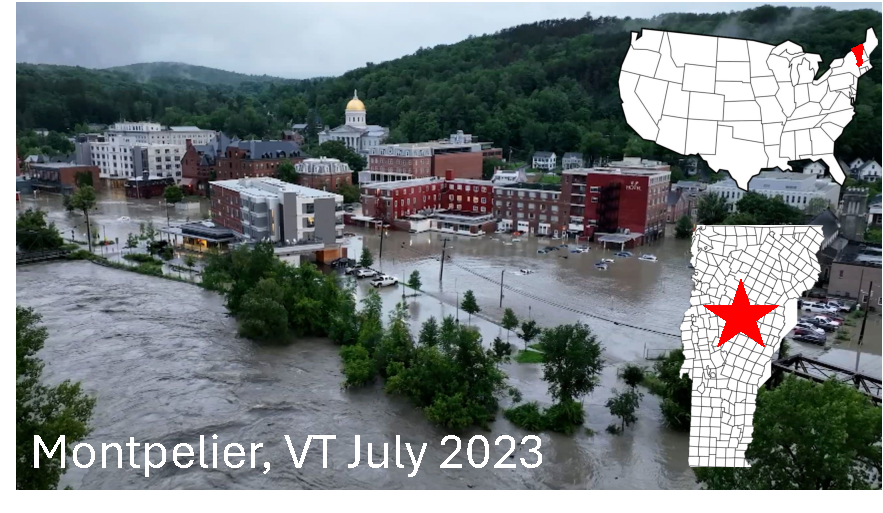
\includegraphics[width=0.45\textwidth]{images/vt.pdf}
\captionsetup{justification=centering,singlelinecheck=false,font=small}
\vspace{-0.9cm}
\caption{Montpelier during the July 2023 flood.}
\label{fig:vt}
\vspace{-0.3cm}
\end{wrapfigure}
\normalsize
Montpelier, Vermont's capital city, experienced catastrophic flooding in July 2023,
with 80\% of its National Register Historic District sustaining damage; it sustained
significant flood damage again in 2024.
The city has experienced over 45 flooding events since 1900 at the confluence of
the Winooski and North Branch rivers.
Its dense downtown core of 19th-century load-bearing masonry commercial buildings,
many pre-dating the 1933 ANSI building code, is the pre-code archetype central to
this proposal.
As Vermont's capital, Montpelier has moderate institutional capacity relative to
comparable communities: a professional emergency manager, Vermont State Historic
Preservation Office support, and a planning department, yet lacks the technical
infrastructure for hydrodynamic simulation.
The framework transfers to any municipality meeting four scope conditions including riverine
flood exposure with inundation persisting long enough for meaningful mass balance
estimation, approximately five or more days; pre-1940 construction representing a
meaningful share of the flood-exposed building inventory; no sustained in-house
hydraulic modeling capacity; and USGS streamflow gauge coverage on the primary
watershed.
%confirm whether the five-or-more-day threshold is the right characterization of what the mass balance model requires for reliable drainage timescale estimation.

\vspace{-10pt}
\subsection{Preliminary results: SAR building-level data, Montpelier 2023 and 2024}

Radar imagery (Synthetic Aperture Radar - SAR) allows us to study flood events, map flooded areas and other surface changes occurring overnight or during storms with dense cloud cover where optical imagery would fail. To properly image transient flood events in details, we need high spatial (~meter-scale or better) and temporal (a few hours) SAR resolution imagery. Open Sentinel-1 (C-band, wavelenght of ~6cm, ~10 meters spatial resolution) and ICEYE (X-band, wavelength of ~3cm, <1m of spatial resolution) data are available over the two Vermont events.
In particular, ICEYE commercial SAR provides building-level flood depth and inundation maps fusing SAR amplitude imagery, with LIDAR and water gauges measurements, at 6-hour temporal resolution for both Montpelier flood events, covering the full inundation and recovery period in each case.
Uncertainty of flood level Katie Iceye? other caveat CW need to mention?
PI Wauthier will process and interpret available SAR imagery from these two sensors, using ICEYE for building-level quantitative measurements and Sentinel-1 for broader flood-extent context given its coarser resolution.  Through a NDA data access agreement, ICEYE data for 271 downtown pre-code masonry buildings, each with ICEYE-measured duration, ICEYE-measured peak depth, and field-recorded damage state, will be analyzed for both the 2023 and 2024 events.
% see with ICEYE what text they want us to add and I think your preliminary screenshots are sufficient for the proposal but we should ask them if OK to include or if they prefer us to include something else with their logo super visible etc. TODO 
The 271-building dataset constitutes the empirical foundation for fragility surface calibration (2023) and held-out validation (2024); the 2024 data is not used in any model fitting (Fig.~\ref{fig:iceye}).

\begin{figure}[h]
\vspace{-0.2cm}
\centering
\begin{subfigure}[b]{0.48\textwidth}
  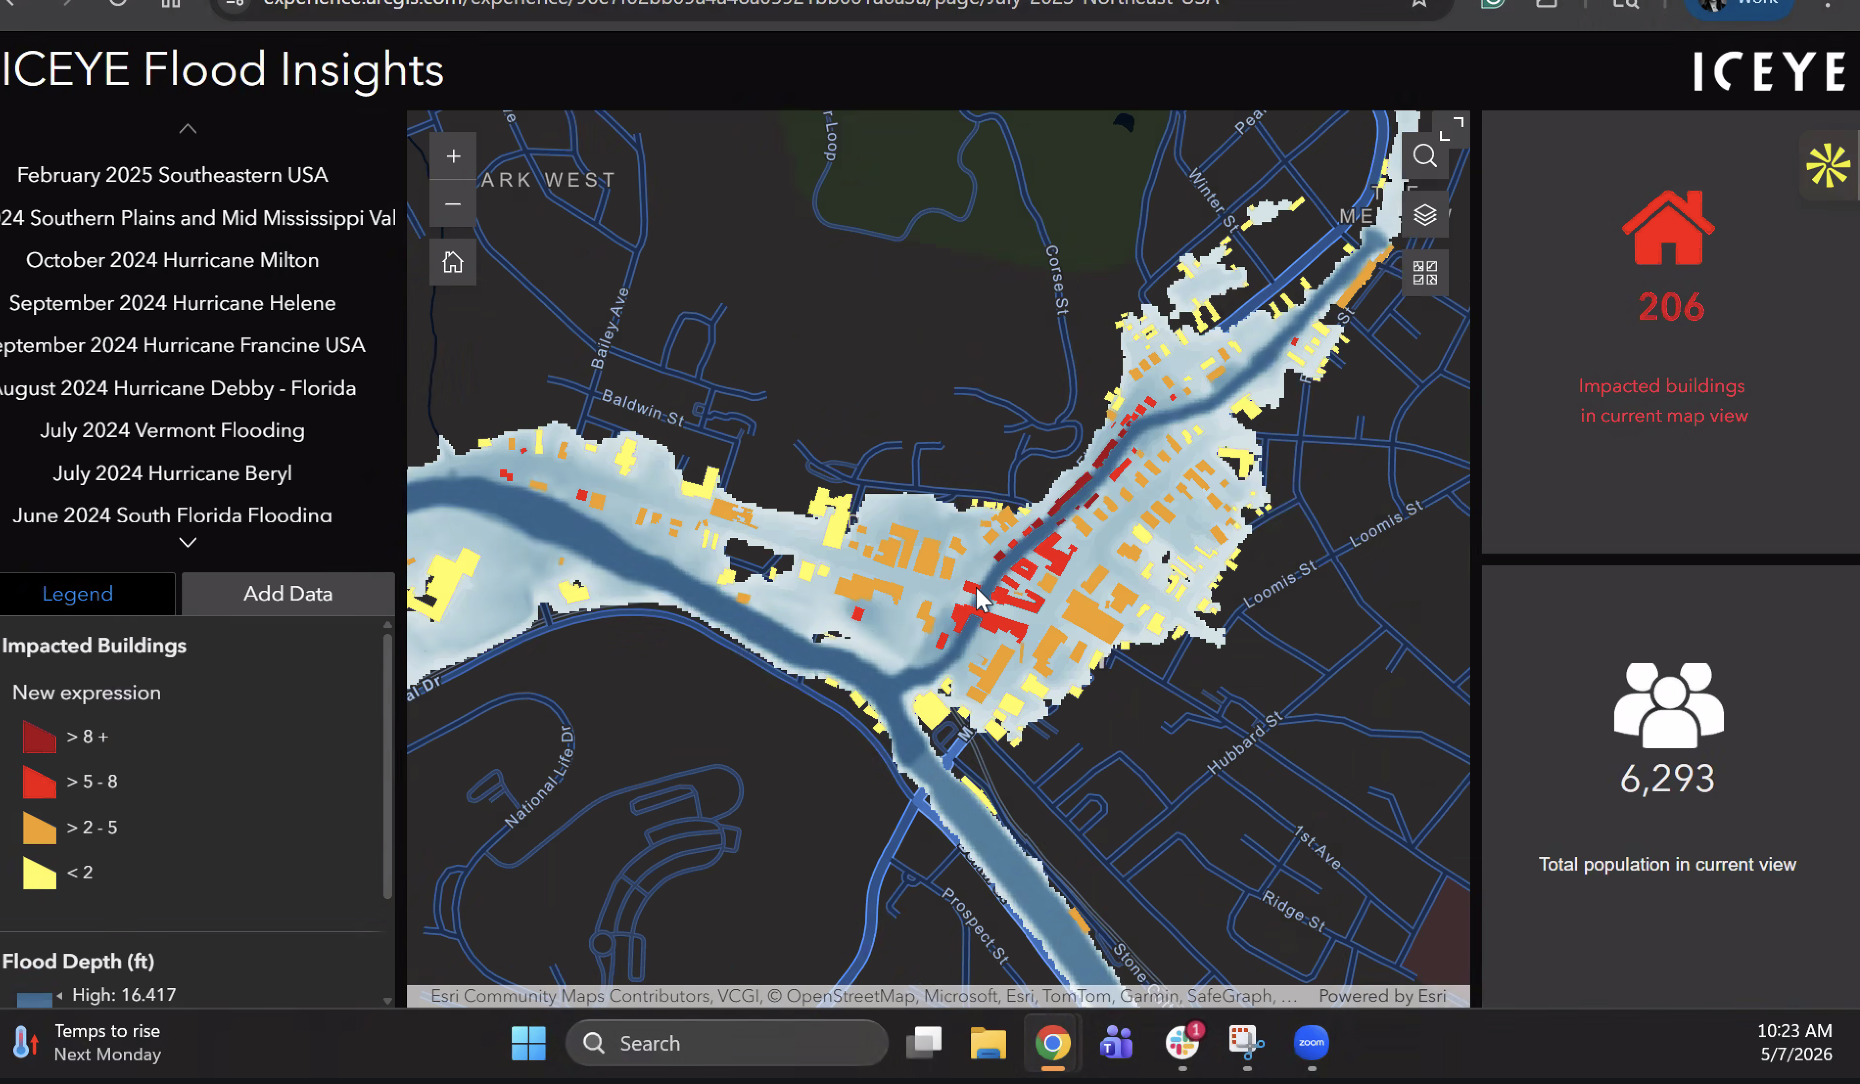
\includegraphics[width=\textwidth]{images/2023.png}
  \captionsetup{font=small}
  \caption{July 2023 (calibration event)}
  \label{fig:iceye_2023}
\end{subfigure}
\hfill
\begin{subfigure}[b]{0.48\textwidth}
  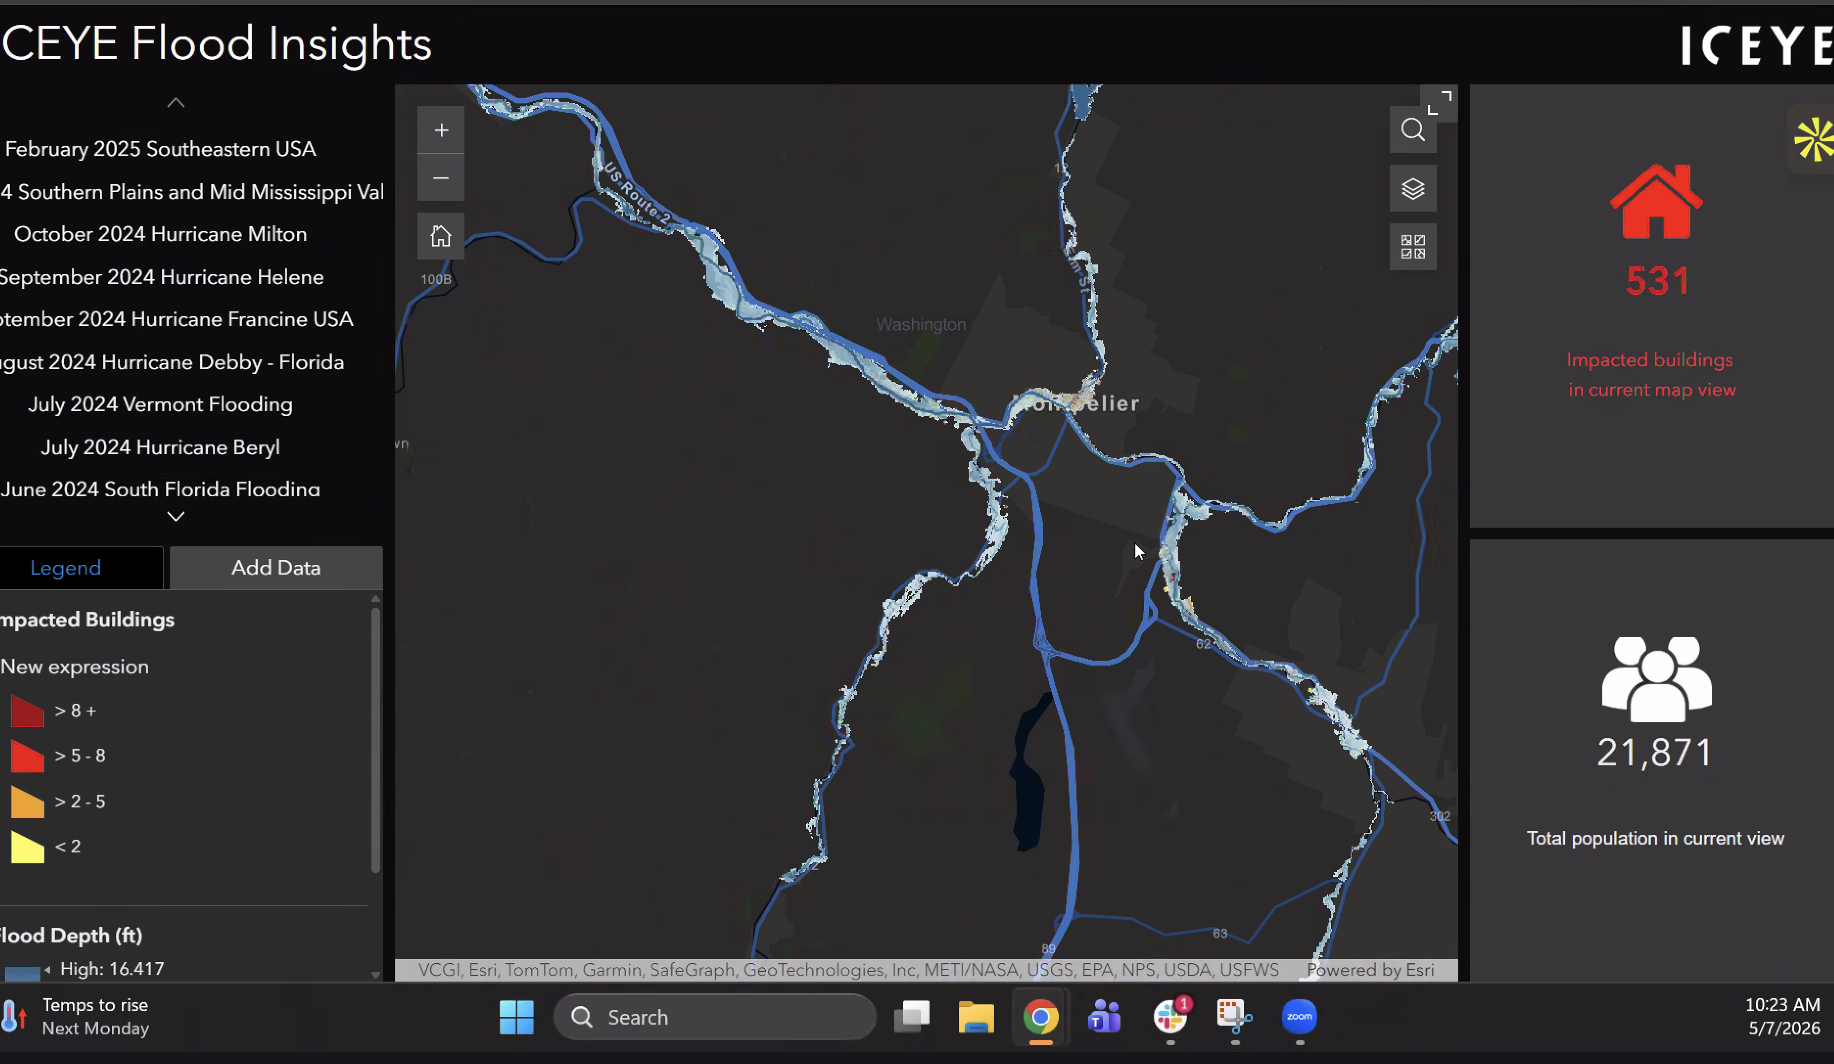
\includegraphics[width=\textwidth]{images/2024.png}
  \captionsetup{font=small}
  \caption{July 2024 (held-out validation event)}
  \label{fig:iceye_2024}
\end{subfigure}
\captionsetup{font=small}
\vspace{-0.3cm}
\caption{ICEYE building-level flood depth, Montpelier downtown core, for both
study events. Building footprints are colored by peak inundation depth (yellow:
$<$2\,ft; orange: 2--5\,ft; red: 5--8\,ft; dark red: $>$8\,ft). PI Wauthier
has separately extracted building-level inundation \textit{duration} at 6-hour
temporal resolution for all 271 buildings across both events; the 2024 event
is held out and not used in any model fitting.}
\label{fig:iceye}
\vspace{-0.3cm}
\end{figure}

% christelle: add 2-3 sentences describing the ICEYE processing pipeline and any flags on the duration and depth measurements.
%
% becca: get the correct figures from company for the full proposal, prob need two panels at the same zoom level: one showing 2023 downtown core (calibration event) and one showing 2024 (held-out validation event).

\subsection{Preliminary results: field damage assessment, Montpelier 2023}
% becca: describe the 2023 field campaign: when it was conducted, the damage state taxonomy (number of states, definitions), methodology for damage state assignment in the field, and the distribution of 271 buildings across damage states. A bar chart of damage state counts and a map of damage state by building footprint would be the strongest figures here.

\subsection{Preliminary results: Winooski mass balance model}
% maggie: describe any preliminary mass balance results for the Winooski watershed that we could cook up: online told me that maybe this would be good but idk what any of this is so its your call--> sub-basin delineation, estimated drainage timescales from the 2023 or 2024 events, comparison of mass balance predictions against USGS gauge records. Order-of-magnitude drainage timescale estimates and a sub-basin map 

% ============================================================
%  RESEARCH PLAN
% ============================================================

\section{Research plan}
RO1 (Napolitano, Wauthier, and Busse) addresses RQ1 through five coupled subtasks:
SAR data processing, interpretation, and error characterization (Wauthier), GIS-parameterizable
mass balance model development (Busse), Bayesian fusion framework development (all
PIs), duration-dependent fragility surface development (Napolitano), and
system validation (all PIs).
RO2 (Napolitano with all PIs) addresses RQ2 through community co-development and
knowledge elicitation (Napolitano), three-mode decision interface co-development
(Napolitano), comparative assessment of community knowledge contribution (all
PIs), and closed-loop validation and protocol transfer (all PIs).

% ── RO1 BOX ──────────────────────────────────────────────────────────────────
\begin{tcolorbox}[colback=mycmykcolor,colframe=black,boxrule=1pt,coltext=black,
  left=1mm,right=1mm,top=1mm,bottom=1mm]
\textbf{Research Objective 1 (RO1, leads: Napolitano, Wauthier, and Busse):
Develop and validate a closed-loop CPS coupling a GIS-parameterizable mass balance
model with community knowledge in a Bayesian framework and duration-dependent
fragility surfaces for pre-code masonry archetypes, and establish whether the system
is decision-adequate for retrofit allocation and pre-storm resource staging without
hydraulic simulation, calibrated on Montpelier 2023 and validated on the held-out
2024 event.}
\end{tcolorbox}

RO1 builds and validates the technical CPS by coupling four components: SAR imagery,
ICEYE commercial SAR for building-level data processing, interpretation,
and error characterization, with open Sentinel-1 SAR for broader flood-extent
context (Subtask~1.1), a
GIS-parameterizable mass balance model (Subtask~1.2), a Bayesian fusion framework
integrating the mass balance prior with community knowledge and the ICEYE-calibrated
likelihood (Subtask~1.3), and duration-dependent fragility surfaces connecting
duration estimates to building damage state probabilities (Subtask~1.4).
ICEYE provides the one-time calibration ground truth for both the likelihood function
and the fragility surface; the operational system runs entirely on USGS gauge data
and NOAA precipitation, which are free and nationally available.
Subtask~1.5 validates the full RO1 system against the 2024 held-out event and
characterizes decision-adequacy across all three operational modes.

\textbf{Subtask 1.1: SAR Data Processing, Interpretation, and Likelihood Characterization
(lead: Wauthier).}
Subtasks 1.1 and 1.2 run in parallel in Year 1: PI Wauthier extracts building-level inundation measurements from ICEYE commercial SAR while PI Busse develops the GIS-parameterized mass balance model; neither depends on the other's output until both feed into the Bayesian fusion framework in Subtask 1.3.
PI Wauthier processes ICEYE commercial SAR data for the 271 downtown Montpelier buildings across both flood events, extracting building-level inundation duration and peak depth at 6-hour temporal resolution and validating building footprint attribution against ground-referenced building inventory.
The key scientific output of this subtask is the empirical error distribution between mass balance predictions and ICEYE-measured duration per building for the 2023 event: how far off the GIS-only model's duration estimate is from what the SAR data actually observed, not a prediction of whether a building floods.
Once Subtask 1.2 delivers $\hat{\tau}_k$ estimates, this error distribution characterizes the systematic and random error of the GIS-parameterized mass balance at building scale and becomes the likelihood in the Bayesian fusion of Subtask 1.3, the statistical model of how ICEYE's measured duration relates to the true duration being estimated, used to update the mass-balance prior.
Open Sentinel-1 imagery will also be processed for both events to provide broader flood-extent context; its ~10\,m resolution is too coarse to resolve individual buildings in the downtown core, so it supports interpretation and cross-checking of the ICEYE-derived building classifications rather than feeding the building-level likelihood directly.

\textbf{Subtask 1.2: GIS-Parameterizable Mass Balance Model (lead: Busse).}
PI Busse develops a hydrological mass balance model for the Winooski watershed above
Montpelier, estimating the drainage timescale $\hat{\tau}_k$ for each building-scale
sub-basin from nationally available GIS layers: watershed delineation and contributing
area from USGS 3DEP and NHD StreamStats, effective impervious fraction from NLCD,
soil infiltration rates from SSURGO, and real-time discharge from USGS station
04288000.
The drainage timescale $\hat{\tau}_k$ represents the expected duration of standing
water under gravitational drainage and serves as the physically grounded prior mean
on inundation duration; the model is designed so that any municipality with a USGS
gauge ID and access to standard national GIS layers can parameterize it without
field data collection.
Inundation duration at building $i$ in sub-basin $k$ is modeled as:
\begin{equation}
  T_i \sim \operatorname{LogNormal}(\mu_i,\; \sigma^2)
\end{equation}
where the log-scale prior mean is:
\begin{equation}
  \mu_i \;=\; \log \hat{\tau}_k \;+\; \delta_i^{\mathrm{comm}}
\end{equation}
$\hat{\tau}_k$ is the mass balance drainage timescale for sub-basin $k$ and
$\sigma^2$ captures residual local drainage uncertainty quantified from historical
Winooski gauge variability.
Subtask~1.2 delivers the GIS-only prior: setting $\delta_i^{\mathrm{comm}} = 0$
gives the baseline model parameterized entirely from national GIS layers, which
constitutes both the operational system for transfer communities and the comparison
baseline for RQ2.
The building-level adjustment $\delta_i^{\mathrm{comm}}$, elicited from community
knowledge in Subtask~2.1 (locally known drainage obstructions, historically slow
routes, anomalous building conditions), augments this baseline in Subtask~1.3;
community knowledge improves the system but is not required to run it.
The LogNormal family is appropriate because duration is strictly positive and
right-skewed; it also maintains dimensional consistency with the log-scale
likelihood in Subtask~1.3.
For pre-storm prediction, NOAA forecast precipitation replaces observed discharge
as the model input; forecast uncertainty is propagated through the mass balance to
produce appropriately wider credible intervals on predicted duration.
% maggie: specify the functional form for tau_k_hat (ratio of stored flood volume to effective channel capacity? Unit hydrograph lag? Something else?). Describe the spatial discretization (approximate sub-basin size), and whether this uses an existing Winooski model or requires new development.
%
% maggie -- IMPORTANT FOR PRE-STORM MODE: Drainage timescale is substantially shorter under dry  conditions than saturated ones; if the mass balance model does  not account for this, pre-storm duration predictions will carry large uncharacterized uncertainty and reviewers may challenge the resource-staging claim in RQ1. Please address explicitly: (1) does the model include an antecedent moisture condition (AMC) input (e.g., AMC-I/II/III from TR-55, or a continuous soil moisture state from SSURGO + prior precipitation)? (2) how is antecedent moisture estimated operationally before a storm (NOAA QPF history? USGS soil moisture network?)? (3) how much does tau_k_hat vary between dry and saturated antecedent conditions for the Winooski if the range is large and the operational estimate is uncertain, the pre-storm credible intervals will be wide enough to limit actionability. If the model handles AMC well, say so since that would strengthens the pre-storm mode substantially. If not, we should narrow the pre-storm claim before submission prob.

\textbf{Subtask 1.3: Bayesian Fusion Framework (leads: Napolitano, Wauthier,
and Busse).}
The Bayesian fusion framework integrates the mass balance prior from Subtask~1.2
with the ICEYE-calibrated likelihood from Subtask~1.1 to produce posterior duration
distributions at each building.
The likelihood characterizes the empirical error between mass balance predictions
and ICEYE ground truth on the log scale, learned from the 2023 calibration event:
\begin{equation}
  \log T_i^{\mathrm{ICEYE}} \mid T_i \;\sim\;
    \mathcal{N}\!\left(\log T_i,\; \sigma_{\mathrm{error}}^2\right)
\end{equation}
where $\sigma_{\mathrm{error}}^2$ is the variance of log-scale mass balance prediction
errors, estimated from the 2023 scatter of $\log\hat{\tau}_k$ versus
$\log T_i^{\mathrm{ICEYE}}$ across all 271 buildings; working on the log scale
maintains dimensional consistency with the LogNormal prior and ensures all duration
quantities remain strictly positive.
$\sigma^2$ and $\sigma_{\mathrm{error}}^2$ are separately identifiable: $\sigma^2$
is pre-estimated from historical Winooski gauge variability independently of the
271-building calibration dataset, while $\sigma_{\mathrm{error}}^2$ is estimated
from the 2023 ICEYE scatter; the two sources are therefore distinct.
Because both the prior and likelihood are Gaussian on the log scale, the posterior
is conjugate and exact: $T_i \mid \log T_i^{\mathrm{ICEYE}} \sim
\operatorname{LogNormal}(\mu_i^*,\; \sigma^{*2})$, where:
\begin{equation}
  \sigma^{*2} \;=\; \left(\frac{1}{\sigma^2} + \frac{1}{\sigma_{\mathrm{error}}^2}
    \right)^{-1}, \qquad
  \mu_i^* \;=\; \sigma^{*2}\!\left(\frac{\mu_i}{\sigma^2}
    + \frac{\log T_i^{\mathrm{ICEYE}}}{\sigma_{\mathrm{error}}^2}\right)
\end{equation}
The posterior mean is a precision-weighted average of the prior mean and the
log-scale SAR observations; buildings in sub-basins where the mass balance has
larger error receive smaller weight on the prior and larger weight on the
observation, and the posterior variance $\sigma^{*2}$ is always narrower than
either variance alone.
Posteriors are computed independently per building; this is a simplification of
the within-sub-basin spatial correlation of inundation durations, and its practical
consequence is that portfolio-level uncertainty across neighboring buildings in the
same sub-basin may be marginally underestimated; for the retrofit ranking decisions
this proposal targets, priority rankings are robust to this approximation.
For operational deployment without SAR imagery, the predictive distribution is
$T_i \sim \operatorname{LogNormal}(\mu_i,\; \sigma^2 + \sigma_{\mathrm{error}}^2)$,
combining prior uncertainty and calibrated mass balance error into a single honest
predictive variance; this wider distribution reflects the full uncertainty of the
system when operating on free data alone.
The 2024 Montpelier event is the held-out test: the calibrated framework, with
all parameters fixed from 2023, is applied to 2024 gauge and NOAA forecast data
and compared against independently collected ICEYE 2024 measurements.

\textbf{Subtask 1.4: Duration-Dependent Fragility Surface Development
(lead: Napolitano).}
Subtask~1.4 requires the processed ICEYE measurements from Subtask~1.1 (building-level
duration and depth for all 271 buildings) and runs in parallel with Subtasks~1.2
and~1.3; it does not depend on the mass balance model.
Duration and peak flood depth are correlated in observational data; this
collinearity is apparent in the Montpelier 2023 dataset and is consistent with
building owner accounts of which structures sustained the most persistent damage
after the July 2023 flood, motivating a two-component approach that separates
the duration effect physically before fitting it statistically.
The \textit{physical component} grounds the duration claim in material science:
component-based analysis of duration-governed degradation mechanisms in pre-code
load-bearing masonry, including mortar softening rate, brick saturation curves,
and rising damp penetration depth as a function of immersion time, provides the
functional form of the duration effect independently of observational confounding.
The \textit{empirical component} calibrates the fragility surface parameters from
field damage observations from the 2023 Montpelier flood, using ICEYE-measured
duration and depth as covariates at building scale for all 271 buildings.
The fragility surface for damage state $ds$ takes the form:
\begin{equation}
  P(DS \geq ds \mid T_i,\; d_i) \;=\; \Phi\!\left(
    \frac{\ln T_i - \lambda_{ds}(d_i)}{\zeta_{ds}}\right)
\end{equation}
where $T_i$ is inundation duration (hours), $d_i$ is peak inundation depth (m),
$\lambda_{ds}(d_i) = \lambda_0 + \gamma \ln d_i$ is the log-scale median duration
capacity (depth shifts the threshold at which duration governs damage), $\zeta_{ds}$
is the log-standard deviation of capacity, and $\Phi$ is the standard normal
cumulative distribution function.
The physical component provides initial estimates of $\lambda_0$, $\gamma$, and
$\zeta_{ds}$; the empirical component refines these parameters from 2023 observations,
and the fitted surface is applied unchanged to 2024 for held-out validation.
The claim under test is that duration adds statistically significant explanatory
power beyond depth alone, evaluated by comparing the bivariate model against a
depth-only baseline using damage prediction accuracy on the 271-building 2024 event.
Because duration and depth are correlated in the 271-building empirical sample, a
depth-only model fit directly to the correlated data could appear competitive with
the bivariate model even where duration has a real physical effect; the
two-component design mitigates this identification problem by anchoring
$\lambda_0$ and $\gamma$ to the physical component's material-science-derived
functional form rather than fitting them from the correlated observations alone.
% becca/napolitano: confirm the identification-strategy specifics before submission -- is a variance inflation factor (VIF) check on the 2023 duration-depth relationship the right diagnostic to report alongside the bivariate-vs-depth-only comparison? Given the 271 buildings are geographically clustered within one downtown core rather than independently sampled, should the comparison use cluster-robust standard errors instead of treating buildings as independent observations? Both are common approaches but need Napolitano's sign-off, not a default insertion.
The posterior $T_i \mid \log T_i^{\mathrm{ICEYE}} \sim
\operatorname{LogNormal}(\mu_i^*, \sigma^{*2})$ from Subtask~1.3 propagates through
Equation~(5) by Monte Carlo integration, producing a building-specific damage state
probability distribution that carries the full inferential uncertainty of the mass
balance and likelihood into the decision layer.
% becca: describe the building archetypes (load-bearing brick URM, stone, timber frame, or combinations); the damage state definitions from 2023 field observations; and the distribution of 271 buildings across damage states.

\textbf{Subtask 1.5: System Validation (leads: all three PIs).}
Subtask~1.5 validates the full RO1 system against the 2024 held-out event across
all three operational modes, with all model parameters fixed from 2023 calibration.
Technical validation compares posterior duration distributions from the Bayesian
framework against SAR and ICEYE 2024 imagery and products for all 271 buildings, reporting root
mean square error, Pearson correlation, and empirical coverage of 90\% credible
intervals; a well-calibrated system should have 90\% of SAR-measured durations
fall within the predicted 90\% credible interval; calibration in the strict
frequentist sense requires repeated experiments, and the 271-building 2024 dataset
constitutes one draw from the event distribution rather than independent trials,
so coverage assessment from a single event is limited; the design maximizes
available power by using all 271 buildings as independent assessment units within
that event, and multi-event calibration assessment is a target for future work.
Damage state validation compares Equation~(5) fragility surface predictions against
2024 field damage observations at building scale, using the posterior duration
distributions as input; the claim under test is that the duration-depth bivariate
model predicts 2024 damage states more accurately than a depth-only baseline fitted
on the same 2023 data.
Decision-adequacy validation assesses whether retrofit priority rankings from the
planning mode align with independent rankings produced by community partners and
domain experts based on direct knowledge of 2024 damage outcomes; alignment is
assessed by rank correlation, and systematic divergence between model rankings and
partner rankings is treated as a finding requiring explanation rather than
suppression.
Pre-storm mode validation applies the framework retrospectively to the 2024 event
using NOAA quantitative precipitation forecast products at 24-, 48-, and 72-hour
lead times before the flood peak; predicted building-level inundation risk maps are
compared against SAR imagery products, and prediction accuracy is reported as a function
of lead time to characterize how forecast uncertainty degrades pre-storm prediction
quality and what actionable lead time the system can reliably provide.
% becca: confirm that 2024 field damage observations will be available for the damage state comparison. Confirm the rank correlation metric for decision-adequacy validation and the composition of the expert panel.

\textbf{Key outcomes:} RO1 produces three primary scientific outputs: a validated
Bayesian framework fusing a GIS-parameterizable mass balance model with community
knowledge priors and an ICEYE-calibrated likelihood, with characterized
decision-adequacy across all three operational modes (Subtask~1.5); the first
empirically derived, duration-dependent fragility surfaces for pre-code
load-bearing masonry archetypes, calibrated on 271 buildings from the 2023
Montpelier flood and validated on the held-out 2024 event (Subtask~1.4); and
a characterization of the conditions under which the GIS-parameterized system
is and is not decision-adequate, including the range of forecast lead times over
which pre-storm predictions remain actionable (Subtask~1.5).

% ── RO2 BOX ──────────────────────────────────────────────────────────────────
\vspace{5pt}
\begin{tcolorbox}[colback=mycmykcolor,colframe=black,boxrule=1pt,coltext=black,
  left=1mm,right=1mm,top=1mm,bottom=1mm]
\textbf{Research Objective 2 (RO2, lead: Napolitano with all PIs): Co-develop
the CPS decision layer with community partners in Montpelier; characterize the
conditions under which locally held community knowledge, entered as Bayesian
calibration priors, improves damage assessment accuracy and calibration relative
to GIS-only model runs; and produce a three-mode decision interface and
transferable protocol for independent community use.}
\end{tcolorbox}

RO2 addresses RQ2 by characterizing the conditions under which community knowledge,
entered as structural calibration input rather than post-hoc validation, improves
the CPS outputs developed in RO1.
Annual co-development workshops in Montpelier (Subtask~2.1) surface locally held
flood knowledge operationalized as Bayesian priors on inundation duration via
$\delta_i^{\mathrm{comm}}$ in Equation~(2).
Subtask~2.2 co-develops the three-mode decision interface with community partners,
shaping criteria, weighting structure, and output format in Year~1 workshops rather
than validating a team-built tool.
Subtask~2.3 runs comparative model versions with and without community-informed
priors to directly quantify the epistemic contribution of community knowledge.
Subtask~2.4 closes the loop through prior updating across events and produces the
transferable protocol.

\textbf{Subtask 2.1: Community Co-Development and Knowledge Elicitation
(lead: Napolitano).}
PI Napolitano leads annual co-development workshops with emergency managers, historic
preservation officials, and building owners in Montpelier across three years.
Community partners include Vermont State Historic Preservation Office representatives,
the Montpelier planning commission, the city emergency manager, and building owners
in the historic downtown core; letters of collaboration from all partners are included
in the supplementary materials.
Building owners participate as primary knowledge sources throughout, not merely as
recipients of decision outputs: their direct observations of which structures held
water longest, which basement entries backed up, and which drainage paths ran clear
constitute the granular building-level knowledge that GIS cannot capture and that
drives the $\delta_i^{\mathrm{comm}}$ adjustments in Equation~(2).
% becca: find 2-3 NSF SCC papers establishing that individuals closest to the problem produce the most actionable knowledge for community technology co-design. The gun violence reduction project (UIUC/City of Champaign, NSF SCC) found that working with youth directly affected by violence, rather than only government stakeholders,  fundamentally changed what the tool needed to do. Similar pattern in the STEM ports  project (rural Maine, NSF SCC): community organizations closest to learners redirected the content focus entirely. Cite 2-3 SCC papers on this from that youtube channel.

\textit{Year~1} workshops begin with a demonstration phase before any knowledge
elicitation.
Prior to the first workshop, the research team builds a working prototype of the
planning-mode interface using the GIS-only mass balance output from Subtask~1.2
and the 2023 ICEYE measurements from Subtask~1.1; this prototype is not the
co-developed interface but the baseline system that shows what GIS data alone
can and cannot predict.
The research team presents this prototype to community partners, showing what the
GIS-only model already knows and, critically, where it visibly errs relative to
what partners know from direct experience; this demonstration-first structure is
designed to earn the trust required for meaningful knowledge elicitation, and the
co-development of the full interface in Subtask~2.2 begins from this baseline
in the same Year~1 workshops.
NSF SCC-funded community technology projects have consistently documented that
communities with repeated exposure to tools that promised to help but required ongoing
effort develop skepticism toward new technical systems; addressing that skepticism
before asking for knowledge commitments is a necessary precondition for genuine
co-development \cite{placeholder_scc_trust}.
% becca: find 2-3 NSF SCC papers documenting technology fatigue and trust-building in community technology adoption. The nutrient management project (Purdue/Illinois Farm Bureau, NSF SCC) found farmers skeptical of "yet another technology" due to  fatigue from prior tools; focus groups revealed this before the team could proceed. The STEM ports project (rural Maine, NSF SCC) found initial partner resistance to  technology in outdoor learning spaces, overcome only after demonstrating that the  tool enhanced rather than replaced existing practice. Cite these and 1-2 others.

Following the demonstration phase, Year~1 surfaces locally held knowledge about which
buildings held water longest, which drainage routes are historically slow, and which
buildings have anomalous conditions; this knowledge is operationalized as
$\delta_i^{\mathrm{comm}}$ in Equation~(2) through a structured two-step protocol.
In the first step, the research team presents the GIS-only model predictions alongside
the 2023 ICEYE duration map; community partners identify buildings where the model is
visibly wrong and characterize the direction and approximate magnitude of the error
(for example, ``this drain always backs up, so this building holds water roughly twice
as long as the model predicts'').
In the second step, relative duration statements are converted to log-scale offsets:
a building estimated to flood twice as long as the model predicts yields
$\delta_i^{\mathrm{comm}} = \log 2 \approx 0.69$; half as long yields
$\delta_i^{\mathrm{comm}} = -\log 2$; buildings where partners have no specific
knowledge receive $\delta_i^{\mathrm{comm}} = 0$, falling back to the GIS-only prior.
Treating $\delta$ as a fixed constant rather than a distribution is an acknowledged
simplification: uncertainty about the magnitude of the adjustment is absorbed into
the posterior's $\sigma^2$ term rather than modeled as a separate hyperprior, which
is conservative and appropriate for a first characterization.
The Year~2 cross-reference of community-stated adjustments against 2023 SAR actuals
provides an empirical validity check on elicitation accuracy before the 2024 held-out
test.
Community partners also co-develop the criteria and weighting structure of the
Subtask~2.2 decision interface and its two output tiers, shaping which investment
outcomes matter most and what level of detail each audience needs; community-identified
priorities are documented in structured form at Year~1 close to enable assessment
of incorporation in subsequent years.
\textit{Year~2} cross-references community-observed building damage reports against
2023 field damage states as a validity check on elicitation, validates framework
outputs against Year~1 stated priorities, and documents discrepancies used to update
the framework architecture.
Year~2 workshops include structured interpretation training in which emergency
managers and planning commission staff learn to read probabilistic damage outputs,
run what-if simulations across the two investment decisions, and interpret pre-storm
risk maps; the training also covers how to present plain-language summaries from the
interface to elected officials and residents without researcher support.
\textit{Year~3} stress-tests the decision interface for independent use across both
output tiers, reassesses whether community priorities have shifted over the project
period, and evaluates whether emergency managers can explain framework outputs to
elected officials and residents without researcher involvement.
This structured process constitutes the \textbf{CIR} component required by NSF~25-543:
locally held knowledge enters the CPS as structural calibration input, community
partners co-develop the framework architecture, and the process is assessed against
documented community-identified priorities throughout.
% becca add approximate workshop participant counts per year,  contact names and titles of Montpelier community partners, IRB coverage status and format (in-person/virtual/hybrid).

\textbf{Subtask 2.2: Three-Mode Decision Interface (lead: Napolitano).}
The decision interface co-developed with community partners supports three operational
modes without requiring any knowledge of mass balance hydrology or Bayesian inference.
Each mode produces two output tiers designed for distinct audiences, a design principle
supported by both NSF SCC-funded community decision support research
\cite{placeholder_scc_twotier} and federal guidance: NIST SP~1310 explicitly identifies
the need for guidance that translates complex infrastructure assessments into simpler
terms for decisionmakers and stakeholders who lack the technical background to interpret
them directly \cite[Sec.~6.1.7.4]{davis2024nist}.
% becca: find 2-3 NSF SCC papers documenting the need for two-tier output design in community technology systems. The human-AI teaming for flood evacuation project  (Clemson/South Carolina, NSF SCC) explicitly found that community members wanted simple binary guidance ("should I evacuate?") while emergency managers wanted technical predictive intelligence with enough depth to brief their superiors.  The Lafayette Parish flood engagement project (NSF SCC) found that simply  providing flood risk information in innovative ways was not enough without also designing for different communication needs across stakeholder groups. Cite these and 1-2 additional SCC papers on differentiated output design.
The \textit{technical tier} presents probabilistic damage state distributions,
credible intervals on duration estimates, ranked retrofit lists, and what-if
simulation outputs for emergency managers and planning commission staff who brief
agency stakeholders, prepare grant applications, and make resource allocation
decisions.
The \textit{plain-language tier} translates the same analysis into a one-page
building risk summary for individual building owners and a district-level investment
comparison for elected officials and residents: for example, "Buildings on Main Street
between Bridge and State have a 67\% probability of damage requiring more than
\$15,000 in repairs in a flood similar to 2023; the proposed retention basin upstream
reduces that probability to 43\% across the district at a cost of \$X per protected
building."
Community partners co-design both tiers in Year~1 workshops, specifying what
information each audience needs to act, not merely what the technical team thinks
should be communicated.

In \textit{planning mode} (always on, no flood required), the technical tier presents
the ranked retrofit priority list and what-if simulations; the plain-language tier
produces the one-page comparisons that emergency managers can hand to elected
officials and building owners without further translation.
In \textit{pre-storm mode} (triggered by incoming NOAA forecast), the mass balance
model runs with forecast precipitation inputs; the technical tier outputs a
building-level inundation risk map with credible intervals; the plain-language tier
outputs a simple color-coded street map and a prioritized resource staging list.
Emergency managers use these outputs to pre-position flood barriers, issue targeted
warnings to specific building owners, and stage response resources before water rises.
In \textit{post-event mode} (after a flood), community members submit structured
damage and drainage observations through the interface; these observations update
$\delta_i^{\mathrm{comm}}$ for the next event, and confirmed drainage retrofits
trigger a recalculation of the affected sub-basin timescale $\hat{\tau}_k$ in the
mass balance model.
The planning and pre-storm modes are prototyped in Year~1 using the GIS-only
prior; the full probabilistic loss calculations below become operational in
Year~2 once the fragility surfaces from Subtask~1.4 and the calibrated posteriors
from Subtask~1.3 are available.
For each retrofit action $a$ under consideration, the framework computes expected
loss by integrating the building damage probability from Equation~(5) over the
posterior duration distribution from Equation~(4):
\begin{equation}
  E[\text{loss} \mid a] \;=\;
  \int_0^\infty \sum_{i}
    P(DS_i \geq ds \mid T,\; d_i,\; a)\cdot L_i
    \cdot p(T \mid T^{\mathrm{ICEYE}},\; a)\; dT
\end{equation}
where $L_i$ is the replacement value at building $i$; the action $a$ modifies both
the fragility (building hardening raises the capacity threshold $\lambda_{ds}$)
and the duration posterior (drainage investment reduces $\hat{\tau}_k$ through
the mass balance model).
Expected loss reduction is one criterion in the multi-criteria decision analysis
score:
\begin{equation}
  S(a) \;=\; \sum_{j=1}^{J} w_j \cdot V_j(a)
\end{equation}
where criteria $V_j$ include structural risk reduction (from Equation~(6)), retrofit
cost, historic preservation value, and community equity; weights $w_j$ are
co-developed with community partners in Year~1 workshops through structured pairwise
comparison.
% becca cnfirm retrofit options in scope (retention basin, channel improvement, flood barriers, foundation waterproofing, masonry repointing?); cost data source (RS Means? FEMA benefit-cost tool?); and the output format co-developed with the community (ranked list, visual map, decision dashboard?).

\textbf{Subtask 2.3: Comparative Assessment of Community Knowledge Contribution
(leads: all three PIs).}
Subtask~2.3 directly addresses RQ2 by running the full CPS under two conditions:
with community-informed priors ($\delta_i^{\mathrm{comm}}$ from Subtask~2.1
workshops) and with GIS-only priors ($\delta_i^{\mathrm{comm}} = 0$), across
all 271 buildings for both flood events.
Posterior duration distributions under each condition are compared against
SAR and ICEYE-measured durations on three metrics: root mean square error, empirical
coverage of 90\% credible intervals (calibration), and damage state prediction
accuracy against 2024 field observations.
Results are disaggregated by building type, drainage sub-basin, and 2023 damage
state to characterize the conditions under which community knowledge and geospatial
data are substitutes versus complements; a building is classified as
community-knowledge-dominant if the $\delta_i^{\mathrm{comm}}$ adjustment moves
the posterior meaningfully toward the SAR observations, and GIS-dominant if the
community adjustment adds no predictive value.
Cases where community knowledge and mass balance predictions conflict and community
knowledge proves correct are the most scientifically informative outcomes; they
identify where GIS cannot see the infrastructure conditions that drive local
drainage behavior, and they constitute the primary evidence for the value of
elicitation investment in future CPS transfer.
Cases where community knowledge underperforms the GIS-only baseline are reported
in full; the conditions under which elicitation adds no value are a scientific
finding, and they directly inform the transfer protocol in Subtask~2.4 by
identifying community contexts where elicitation effort is not warranted.
% becca consider reporting continuous ranked probability score (CRPS) as a proper scoring rule for probabilistic outputs alongside RMSE. Confirm that   the full substitutes-versus-complements results, including null findings, will be published.

\textbf{Subtask 2.4: Closed-Loop Validation and Transferable Protocol
(leads: all three PIs).}
The closed loop closes through Bayesian prior updating across events rather than
post-retrofit physical detection.
After each flood event, structured community observations submitted through the
post-event mode update $\delta_i^{\mathrm{comm}}$ for affected buildings;
buildings whose observed durations consistently exceed or fall below mass balance
predictions in the same direction receive updated prior means that carry forward
to the next event.
After drainage retrofit completion, Co-PI Busse updates $\hat{\tau}_k$ directly
from the engineering specifications of the completed work: a retention basin of
known storage volume and outlet capacity changes the drainage timescale by a
calculable amount, so the parameter is updated from design drawings rather than
a full GIS model re-run; after building hardening retrofits, the fragility
capacity threshold $\lambda_{ds}$ is updated for the retrofitted structures.
No drainage retrofits are currently planned in Montpelier; Montpelier community
partners are open to investment based on the findings of this research, and the
Year~3 decision interface is designed to produce the probabilistic comparison of
drainage investment versus distributed building hardening that would inform that
decision.
The retrofit update pathway is therefore demonstrated computationally within the
grant period: the research team will simulate a plausible drainage investment
scenario in Subtask~2.4, update $\hat{\tau}_k$ from the engineering
specifications of that scenario, and show the resulting change in posterior
duration distributions and retrofit priority rankings.
The 2024 event provides the first empirical test of whether one event cycle of
community observation updates measurably improves posterior accuracy relative to
the 2023-only calibration baseline.
The transferable protocol specifies the minimum pathway for a new community:
a USGS gauge ID, standard national GIS layer downloads (USGS 3DEP, NLCD, SSURGO,
NHD StreamStats), and one co-development workshop to elicit initial
$\delta_i^{\mathrm{comm}}$ values, optionally supported by free Sentinel-1 imagery
as a rough visual aid for flood-extent discussion where local recall is difficult,
combined with the open-source software package
initialized from Montpelier-derived mass balance and fragility parameters.
A community operating under this protocol will have wider credible intervals than
Montpelier because it lacks local ICEYE calibration; access to free Sentinel-1
imagery does not close this gap, since its coarser resolution cannot support
building-level calibration, so credible intervals remain at the transferred
default width regardless of whether open SAR imagery is available locally.
The expected interval widths,
derived from the $\sigma_{\mathrm{error}}^2$ characterization in Subtask~1.1, are
reported as part of the protocol documentation so communities can assess
decision-adequacy before committing to adoption, and intervals narrow with each
community observation cycle.
% becca / maggie confirm the engineering specification approach for updating tau_k_hat -- what inputs does Maggie need from a retrofit design drawing  to compute the change in drainage timescale? Storage volume + outlet capacity? Confirm the computational scenario for Subtask 2.4 (what  retention basin size / location is plausible for Montpelier based on   the watershed geometry?).

\textbf{Key outcomes:} RO2 produces three primary outputs: a three-mode decision
interface independently operated by Montpelier community partners in Year~3, with
two output tiers co-developed with emergency managers, historic preservation
officials, and building owners (Subtask~2.2); a direct characterization of the
conditions under which community knowledge and geospatial data are substitutes
versus complements in CPS calibration, including cases where community knowledge
adds no value relative to the GIS-only baseline (Subtask~2.3); and a transferable
co-design protocol released alongside the open-source software package, enabling
any municipality with a USGS gauge and standard GIS access to initialize the system
from one workshop without a commercial SAR purchase (Subtask~2.4).
% resolved 2026-07-22 per Christelle: Sentinel-1's resolution is too coarse for building-level detail but fine for rough/qualitative flood-extent context. Added as an optional workshop visual aid in the transferable-protocol paragraph above (Subtask~2.4).

\begin{figure}

\includegraphics[width=0.6\textwidth]{images/img.jpg}
\captionsetup{justification=centering,singlelinecheck=false,font=small}
\caption{\placeholder{Project timeline (Gantt chart) with PI assignments.}}
\label{fig:timeline}
\end{figure}

% ============================================================
%  BROADER IMPACTS
% ============================================================

\section{Broader impacts}

The closed-loop CPS framework transforms how flood-affected communities interact
with infrastructure risk, providing the probabilistic damage assessments and
pre-storm decision support that small, resource-constrained municipalities need
to evaluate building retrofits and drainage investments where no such pathway
currently exists.
By enabling better-informed retrofit investment decisions, the framework directly
improves the quality of life of residents who live, work, and rebuild in
repeatedly-flooded historic communities, reducing the flood damage burden that
falls disproportionately on towns with the fewest resources to recover.
The planning mode is available from the day of deployment, before a new flood
occurs; the pre-storm mode provides actionable building-level risk information
before water rises; the post-event mode makes the system more accurate with each
event, all without any proprietary data or ongoing research support.

The framework's operational sensing layer requires only USGS gauge data and NOAA
precipitation, both free and nationally available;
the mass balance model is parameterizable from USGS 3DEP, NLCD, SSURGO, and NHD
StreamStats for any municipality with a gauge.
% resolved 2026-07-22 per Christelle: yes, this is the point -- SAR (as a suite, not ICEYE exclusively) is a one-time calibration input to Maggie's mass balance model, not a recurring operational requirement, so a new community never needs to buy its own SAR data.
A new community needs a gauge ID, standard GIS access, and one community workshop
to elicit local drainage knowledge; no commercial SAR purchase, no hydrologist, and no
hydraulic model is required.
% becca: quantify the transferable community count using FEMA NFIP enrollment data (riverine flood communities), ACS table B25035 (pre-1940 housing stock),   USGS NWIS (gauge coverage), and FEMA DFIRM (communities without hydraulic   models). Convert the implied "thousands of towns" claim into a bounded, citable estimate.

Emergency managers, historic preservation officials, and planning commission staff
gain structured capacity to interpret probabilistic damage assessments, use forecast
inputs for pre-event resource staging, and run what-if simulations for investment
decisions independently.
The CIR co-development methodology, documented as a transferable protocol, advances
CPS practice by establishing how structured elicitation of locally held flood
knowledge can be translated into informative Bayesian prior distributions, making
resident knowledge measurably load-bearing in model calibration rather than
supplementary narrative input.
Graduate students will receive cross-disciplinary training spanning
SAR imagery data processing (Co-PI Wauthier), hydrological mass balance modeling
and GIS-parameterized watershed analysis (Co-PI Busse), and probabilistic structural
assessment and community-engaged research (PI Napolitano).
% becca: name the xxx PhD students, their advising assignments, and any co-advising.

\vspace{-10pt}
\subsection{Potential for transformative impact}
This framework is the first to place community-scale drainage investments and
individual building retrofits on the same probabilistic basis for small historic
municipalities, resolving an investment allocation problem that annually re-injures
these communities without resolution.
The generalizable CPS architecture principle, that free geospatial data fused with
community knowledge is sufficient for the specific investment decisions
resource-constrained municipalities face, applies beyond flood resilience to any
infrastructure domain where national data layers and community knowledge are available
but simulation is not.
The characterization of when community knowledge and geospatial data are substitutes
versus complements has direct implications for how CPS research treats locally held
knowledge across socio-technical systems far beyond flood risk.

\vspace{-10pt}
\subsection{Education and broadening participation}

In addition to broader impacts for study communities, the project integrates research
outcomes into engineering education.
% becca: describe the xxx PhD students total across the three PIs, their institutions,   research assignments by RO, and any cross-college co-advising plan.

Undergraduate students hired for this project will participate in the Building
Engineering Seminal Undergraduate Research Experience (BESURE) program at Penn State
% becca add

\vspace{-10pt}
\subsection{Open science and transferability}
The Bayesian fusion code, mass balance parameterization pipeline, and decision
interface will be released on GitHub under an MIT license, with full documentation
enabling any municipality to initialize the system from national GIS data layers.
Derived SAR imagery, codes, and building-level inundation products for Montpelier will be shared on
DesignSafe-CI; field damage state observations and community workshop documentation
will be shared on the Open Science Framework with appropriate anonymization.
The community knowledge elicitation protocol will be released alongside the technical
software as a transferable co-design artifact: gauge ID, GIS downloads, one workshop.

% ============================================================
%  PROJECT TIMELINE AND EVALUATION
% ============================================================

\section{Project timeline and evaluation}

Progress will be monitored through monthly PI team meetings and annual project
reviews.
The three-year project runs RO1 technical development (Subtasks~1.1 through~1.4)
in Years~1 and~2 in parallel with RO2 Year~1 co-development workshops and
decision interface construction; system validation (Subtask~1.5) and comparative
assessment (Subtask~2.3) run in Year~2 following 2023 calibration; closed-loop
validation and protocol transfer (Subtask~2.4) conclude in Year~3 concurrent with
Year~3 independent-use stress testing.
The project includes a formal assessment component evaluating success across three
dimensions, with the following key performance indicators.
\textit{Technical KPIs} (Subtask~1.5): RMSE on building-level duration estimates
against 2024 SAR imagery products at or below the threshold at which ranking uncertainty affects
retrofit priority decisions; empirical coverage of 90\% credible intervals between
0.85 and 0.95 across 271 buildings; damage state prediction accuracy of the
duration-depth bivariate model exceeding the depth-only baseline by a statistically
significant margin on the 2024 held-out event; pre-storm mode producing actionable
building-level risk rankings at 48-hour forecast lead time.
\textit{Community engagement KPIs} (Subtask~2.1): proportion of Year~1 stated
community priorities reflected in Year~2 framework outputs, evaluated by community
partners in Year~2 workshops with all discrepancies documented and addressed before
Year~3; structured elicitation producing $\delta_i^{\mathrm{comm}}$ values for
at least 80\% of the 271 buildings by end of Year~1.
\textit{Community knowledge contribution KPIs} (Subtask~2.3): community-informed
model achieves lower RMSE and better calibration than the GIS-only baseline on at
least one disaggregated sub-group; substitutes-versus-complements characterization
published with full results including null findings.
\textit{Adoption KPIs} (Year~3): emergency managers successfully operate all three
decision interface modes without researcher support in the Year~3 stress test;
emergency managers demonstrate ability to explain pre-storm risk maps and
planning-mode retrofit comparisons to elected officials and residents without
researcher involvement.
% becca: confirm the RMSE threshold for "decision-adequate" duration estimation....this requires a judgment about how much duration estimation error changes retrofit priority rankings; a sensitivity analysis on the 2023 data before   submission would let us set this threshold defensibly...? is this worth it?

% ============================================================
%  RESULTS FROM PRIOR NSF SUPPORT
% ============================================================

\vspace{-10pt}
\section{Results from prior NSF Support}

\noindent\textbf{PI Napolitano:}
% becca: add prior NSF support in this format:
%   (a) award number, dollar amount, dates
%   (b) title
%   (c) intellectual merit (2-3 sentences), broader impacts (2-3 sentences)
%   (d) publications (cite key list)
%   (e) publicly shared datasets
%   (f) renewal status

\noindent\textbf{Co-PI Wauthier:}
Christelle Wauthier is the PI on NSF EAR-1945417 (\$499,999k, 08/01/20-07/31/26): “CAREER: Numerical Modeling of Volcanic Flank Instability Processes”. Intellectual Merit: This CAREER proposal addresses why the style, behavior, and timing of the cyclic growth then destruction of volcanic edifices varies across such a wide spectrum. It focuses on flank collapse on ocean island volcanoes and in using modeling to unravel the observed complexity in data sets representing a spectrum of type volcanoes. Broader Impacts: Graduate and undergraduate education, support for underrepresented undergraduate research interns, new educational activities, and FEM and other modeling training for graduate students. Research products: Cooper et al., 2023; Leeburn* et al., 2022; Gonzalez-Santana* et al., 2022, 2024; Gonzalez-Santana* and Wauthier, 2021; Poppe* et al., 2024; Kim* et al., 2024; Wauthier and Ho, 2024; Gonzalez-Santana* et al., 2025, all of which are listed in the References.


\noindent\textbf{Co-PI Busse:}
\textbf{Co-PI Busse:} is senior personnel on NSF CBET-2400672 (\$1,000,000, 8/2024 - 7/2029):
"RAISE: CET: Co-development of engineering energy literacy and engineering identities through campus decarbonization research."
Intellectual Merit:
This work integrates six component-specific research directions to address fundamental questions associated with net-zero fuels in the context of Combined Heat and Power (CHP) decarbonization.
Intellectual Merit of the research lies in the integrated real-world system evaluation approach as well as the evaluation of student energy literacy through their research experience. 
Broader Impacts:
The Broader Impacts include advancement of decarbonization technologies and the development of an energy-literate future engineering workforce.  
Research Products: None.
% maggie: add prior NSF support in this format:
%   (a) award number, dollar amount, dates
%   (b) title
%   (c) intellectual merit (2-3 sentences), broader impacts (2-3 sentences)
%   (d) publications (cite key list)
%   (e) publicly shared datasets
%   (f) renewal status

\newpage
\bibliography{biblio.bib}

\end{document}

